% !TEX root = ../../main.tex

\section{Nitrogen sorption isotherms}\label{appx:def:n2phys}

\FloatBarrier%
\subsection{DMF leached samples}
\begin{figure}[!h]
    \centering

    \begin{subfigure}{0.4\linewidth}
        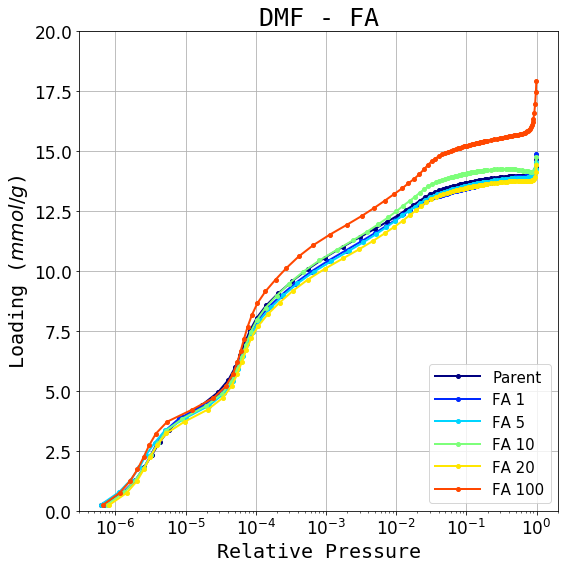
\includegraphics[width=\textwidth]{n2phys/dmf-fa}%
        \label{appx:def:fgr:n2phys-dmf-fa}
    \end{subfigure}
    \begin{subfigure}{0.4\linewidth}
        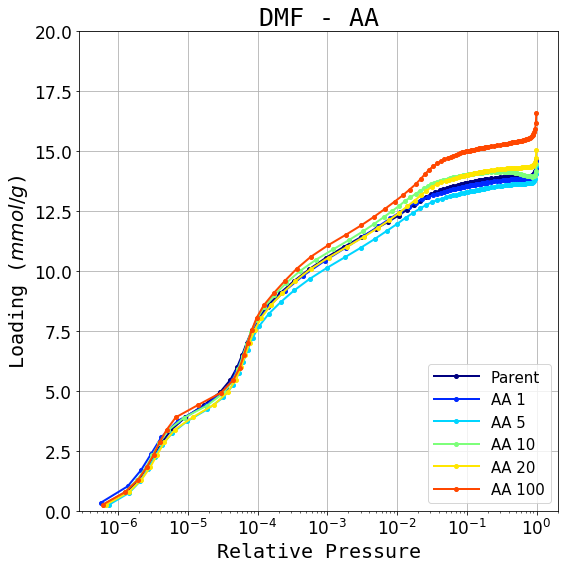
\includegraphics[width=\textwidth]{n2phys/dmf-aa}%
        \label{appx:def:fgr:n2phys-dmf-aa}
    \end{subfigure}
    
    \begin{subfigure}{0.4\linewidth}
        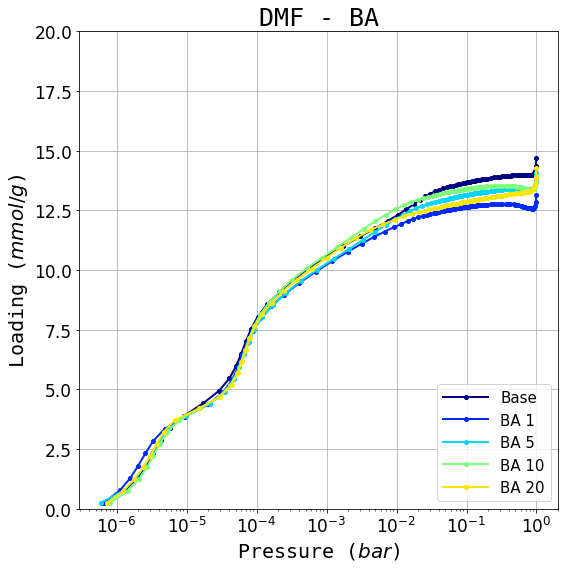
\includegraphics[width=\textwidth]{n2phys/dmf-ba}%
        \label{appx:def:fgr:n2phys-dmf-ba}
    \end{subfigure}

    \caption{DMF isotherm dataset activated at \SI{200}{\degreeCelsius}}%
    \label{appx:def:fgr:n2phys-dataset}
    
\end{figure}

\FloatBarrier%
\pagebreak
\subsection{\ce{H2O} leached samples}
\begin{figure}[!h]\ContinuedFloat{}
    \centering

    \begin{subfigure}{0.4\linewidth}
        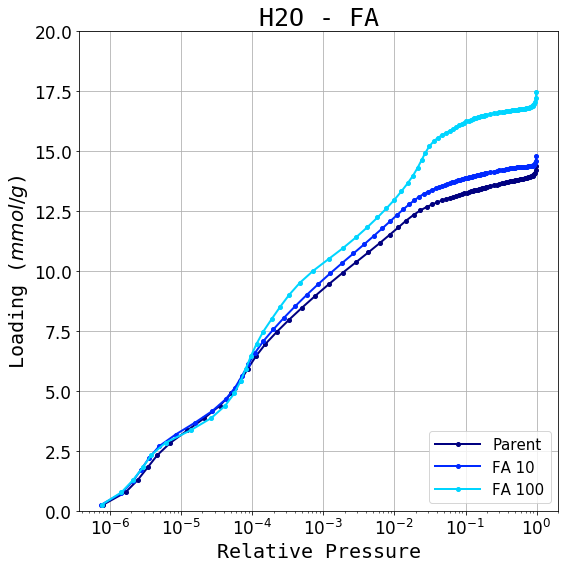
\includegraphics[width=\textwidth]{n2phys/h2o-fa}%
        \label{appx:def:fgr:n2phys-h2o-fa}
    \end{subfigure}
    \begin{subfigure}{0.4\linewidth}
        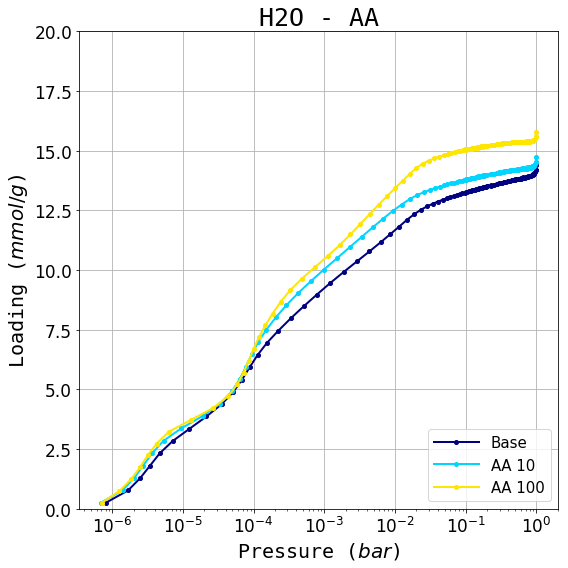
\includegraphics[width=\textwidth]{n2phys/h2o-aa}%
        \label{appx:def:fgr:n2phys-h2o-aa}
    \end{subfigure}
    
    \begin{subfigure}{0.4\linewidth}
        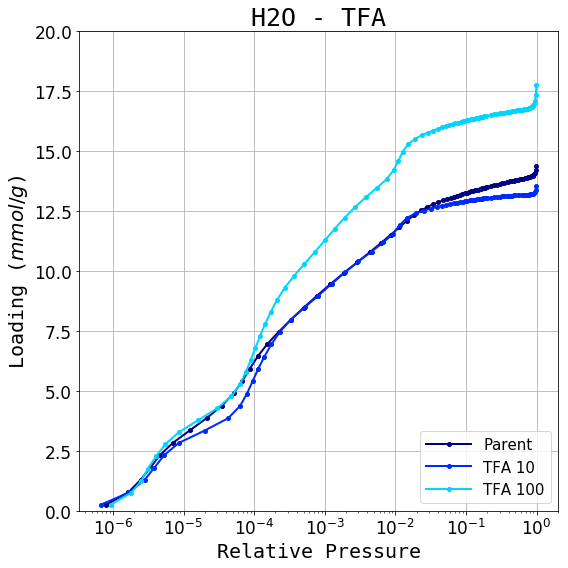
\includegraphics[width=\textwidth]{n2phys/h2o-tfa}%
        \label{appx:def:fgr:n2phys-h2o-tfa}
    \end{subfigure}

    \caption{\ce{H2O} isotherm dataset activated at \SI{200}{\degreeCelsius}}%
    
\end{figure}

\FloatBarrier%
\pagebreak
\subsection{MeOH leached samples}
\begin{figure}[!h]
    \centering
    \begin{subfigure}{0.4\linewidth}
        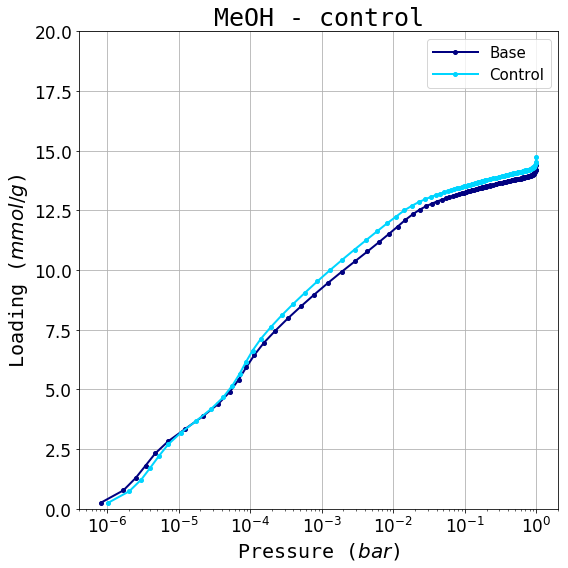
\includegraphics[width=\textwidth]{n2phys/meoh-control}%
        \label{appx:def:fgr:n2phys-meoh-cont}
    \end{subfigure}
    \begin{subfigure}{0.4\linewidth}
        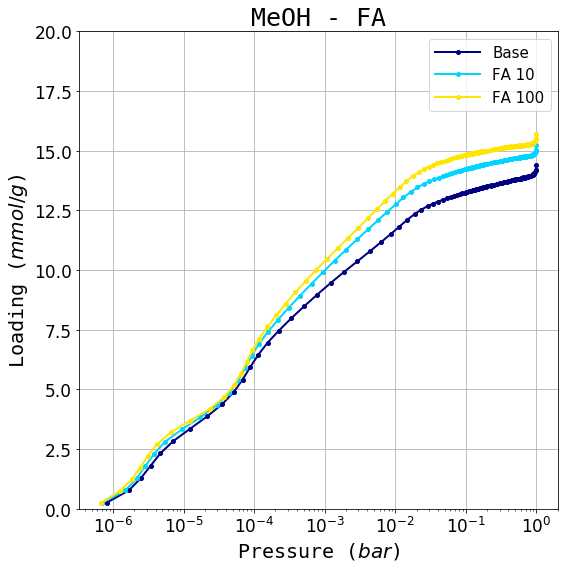
\includegraphics[width=\textwidth]{n2phys/meoh-fa}%
        \label{appx:def:fgr:n2phys-meoh-fa}
    \end{subfigure}

    
    \begin{subfigure}{0.4\linewidth}
        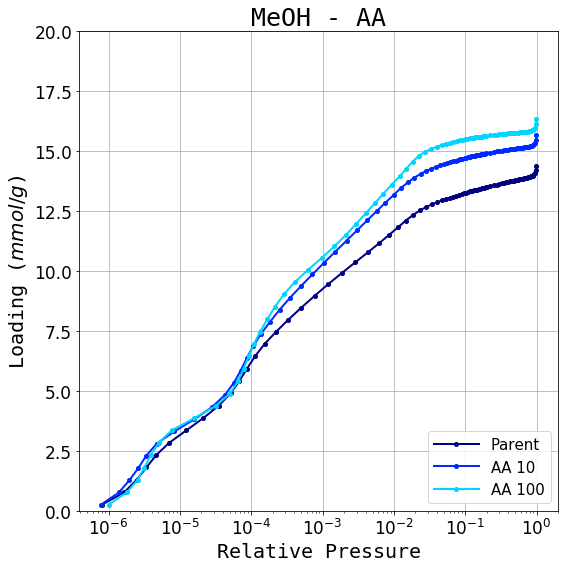
\includegraphics[width=\textwidth]{n2phys/meoh-aa}%
        \label{appx:def:fgr:n2phys-meoh-aa}
    \end{subfigure}
    \begin{subfigure}{0.4\linewidth}
        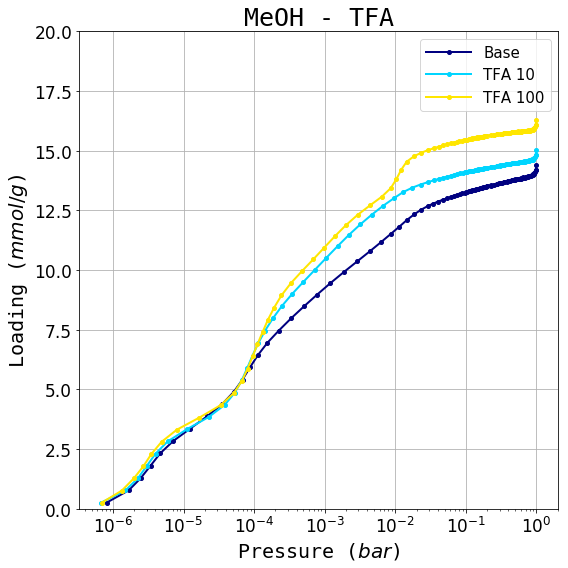
\includegraphics[width=\textwidth]{n2phys/meoh-tfa}%
        \label{appx:def:fgr:n2phys-meoh-tfa}
    \end{subfigure}

    \begin{subfigure}{0.4\linewidth}
        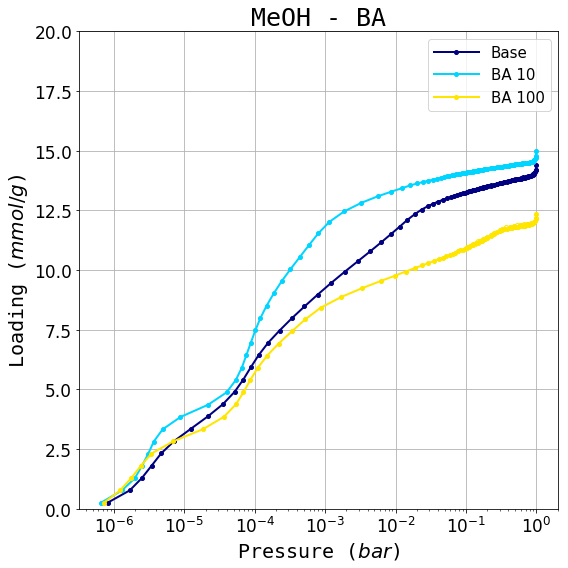
\includegraphics[width=\textwidth]{n2phys/meoh-ba}%
        \label{appx:def:fgr:n2phys-meoh-ba}
    \end{subfigure}

    \caption{MeOH isotherm dataset activated at \SI{200}{\degreeCelsius}}%
    
\end{figure}

\FloatBarrier%
\pagebreak
\subsection{DMSO leached samples}
\begin{figure}[!h]
    \centering
    \begin{subfigure}{0.4\linewidth}
        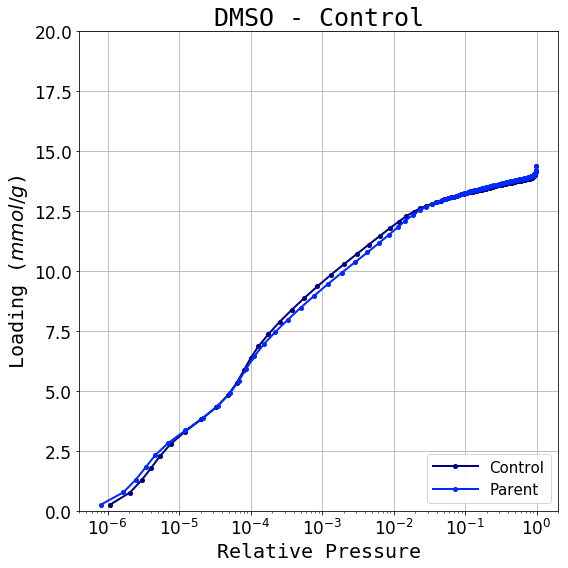
\includegraphics[width=\textwidth]{n2phys/dmso-control}%
        \label{appx:def:fgr:n2phys-dmso-cont}
    \end{subfigure}
    \begin{subfigure}{0.4\linewidth}
        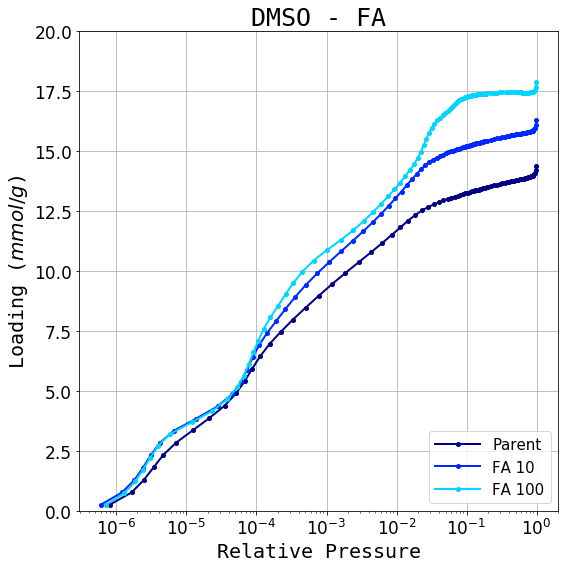
\includegraphics[width=\textwidth]{n2phys/dmso-fa}%
        \label{appx:def:fgr:n2phys-dmso-fa}
    \end{subfigure}

    
    \begin{subfigure}{0.4\linewidth}
        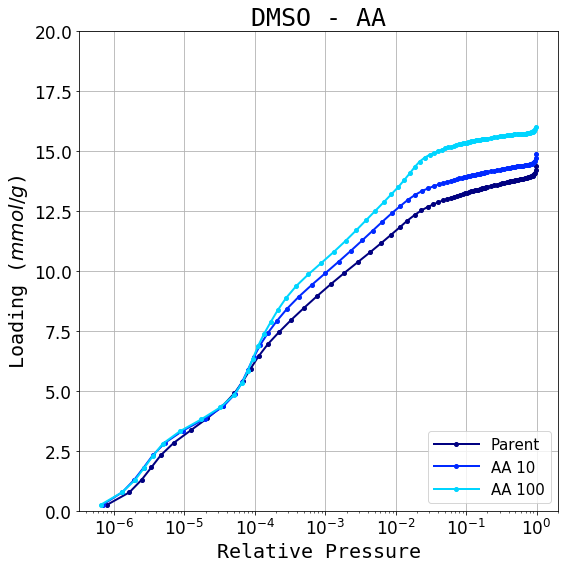
\includegraphics[width=\textwidth]{n2phys/dmso-aa}%
        \label{appx:def:fgr:n2phys-dmso-aa}
    \end{subfigure}
    \begin{subfigure}{0.4\linewidth}
        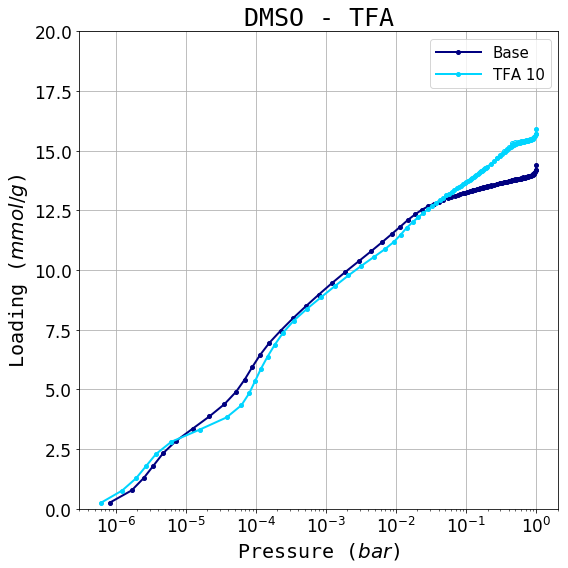
\includegraphics[width=\textwidth]{n2phys/dmso-tfa}%
        \label{appx:def:fgr:n2phys-dmso-tfa}
    \end{subfigure}

    \begin{subfigure}{0.4\linewidth}
        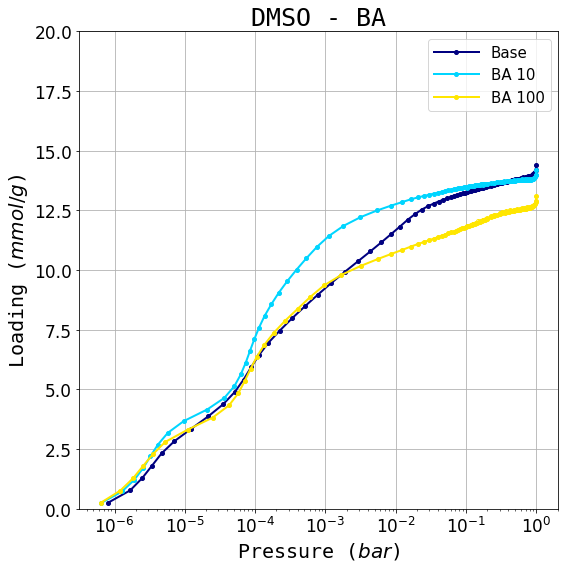
\includegraphics[width=\textwidth]{n2phys/dmso-ba}%
        \label{appx:def:fgr:n2phys-dmso-ba}
    \end{subfigure}

    \caption{DMSO isotherm dataset activated at \SI{200}{\degreeCelsius}}%
    
\end{figure}